\chapter{Architecture Study}

This study's main purpose is to figure out how suited each architecture is for \gls{ADT}, more specifically \gls{DTM} tasks. This could help us figure out which architecture is superiour for \gls{ADT}, if there are any similarities between architectures who perform similarly well, or if there are any architectures who perform poorly.

\section{Methodology}

We perform hyperparameter tuning and model selection to train a separate model for each architecture over each dataset. At last we test the model on each dataset's respective test split. As a result, we are left with performance measures on unseen data from the same distribution as those each model was train on. This will give us a good intuition into each architecture's ability to learn the task of \gls{ADT} and could help us estimate their generalization ability.

\section{Results}	

\begin{table}[H]
    \centering
    \hspace*{-0.6cm}
    \begin{tabular}{l|cccc}
        Architecture & ENST+MDB & E-GMD & Slakh & ADTOF-YT       \\
        \hline
        Recurrent Neural Network	& 0.6682 &	0.889 &	0.864 &	\textbf{0.9635} \\
        Convolutional Neural Network	& 0.7797 &	0.8744 &	0.8318 &	0.844 \\
        Convolutional Recurrent Neural Network	& \textbf{0.8132} &	\textbf{0.8935} &	\textbf{0.8959} &	0.9333 \\
        Convolutional Transformer	& 0.776 &	0.8831 &	0.8826 &	0.9535 \\
        Vision Transformer	& 0.5426 &	0.8779 &	0.879 &	\textbf{0.9635} \\
        
    \end{tabular}
    \caption{The Micro F1-score for each architecture, trained and tested on each dataset. The performances which are bolded represent the highest F1-score, and thus best performance, for that respective dataset.}
    \label{ArchitectureResultsTable}
\end{table}


\begin{figure}[H]
    \centering
    \hspace*{-0.8cm}
    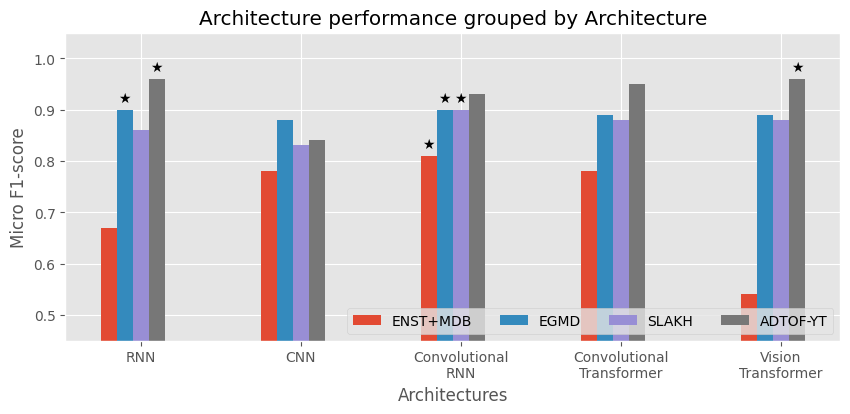
\includegraphics[scale=0.8]{figures/architectureperformancearchitecture.png}
    \caption{The Micro F1-score of each architecture on each dataset, displayed in a bar-plot and grouped by architecture. A ($\star$) over the bar denotes that it is the best performing architecture for that respective dataset.}
    \label{ArchitectureResultsArchitectureFigure}
\end{figure}

\begin{figure}[H]
    \centering
    \hspace*{-0.8cm}
    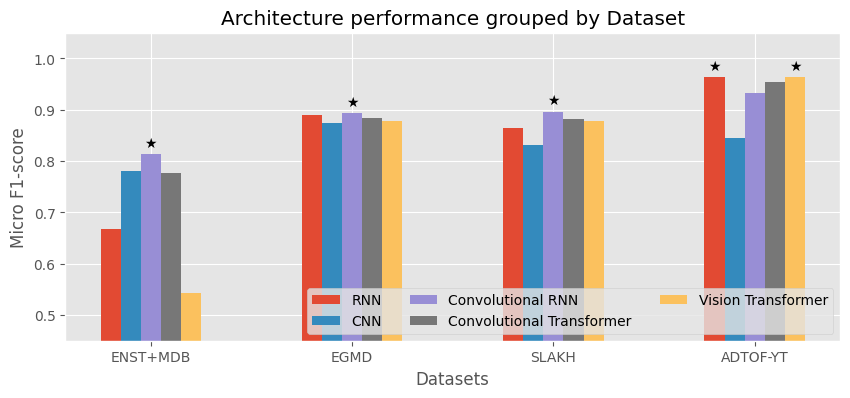
\includegraphics[scale=0.8]{figures/architectureperformancedataset.png}
    \caption{The Micro F1-score of each architecture on each dataset, displayed in a bar-plot and grouped by dataset. A ($\star$) over the bar denotes that it is the best performing architecture for that respective dataset.}
    \label{ArchitectureResultsDatasetFigure}
\end{figure}

\section{Discussion}

As we can see...